
Although the body of literature in the area of proposed research is not
expansive, there have been a number of relevant studies. These, in some way,
are related to the the prediction of forensics-applicable categories or
quantities of nuclear materials using statistical methods.  With regards to
broader forensics capabilities, materials from different steps of the nuclear
fuel cycle are being studied.  Even though each material has its own forensics
signatures, the process of applying statistical methods to the analysis of
material provenance is similar for each. 

For example, on the front end of the fuel cycle, an entity may have obtained
\gls{UOC} if they have enrichment capabilities.  One study performed
statistical analyses on \gls{UOC} from 21 sources (throughout seven countries)
using 30 concentration measurements of various elements, isotopes, and
compounds, e.g., sodium, magnesium, thorium, uranium-234, or halide compounds
\cite{robel_2009}.  The goal of classifying the source and the country was
reached 60\% and 85\% of the time, respectively, with the unique method
developed in the paper (an iterative partial least squares discrimination
analysis approach), which outperformed decision trees and \textit{k}-nearest
neighbors.
%Note: there was a ton of skew in their data and the correction for that was
%weak sauce

On the back end, an organization might have interest in \gls{SNF} if they have
reprocessing capabilities.  Or, perhaps already separated plutonium from
\gls{SNF} has been intercepted and needs to be traced. Another study addresses
this by performing factor analysis on theoretical separated plutonium from
various sources of \gls{ORIGEN}-simulated \gls{SNF} based on their composition
at the end of irradiation \cite{nicolaou_pu}.  Since in this study all
materials are the same age, five plutonium isotopes ($A = 238-242$) correctly
predicted a test sample. However, taking different times since irradiation and
reprocessing into account requires more isotopic measurements. 

\subsection{Factor Analysis Work}

In addition to the immediately aforementioned work, there is a suite of work on
performing classification using factor analysis or isotopic ratios in
combination with visual distinction.  Although factor analysis explicitly
requires the input of domain knowledge, it is a valuable first step towards
understanding how statistical methods can provide insightful models to classify
materials.  This series of work seeks to accomplish classification of a reactor
history (reactor type, enrichment, burnup) using the distinguishability between
similar sets of samples, as pictured in Figure \ref{fig:nico}.

\begin{figure}[!htb]
  \centering
  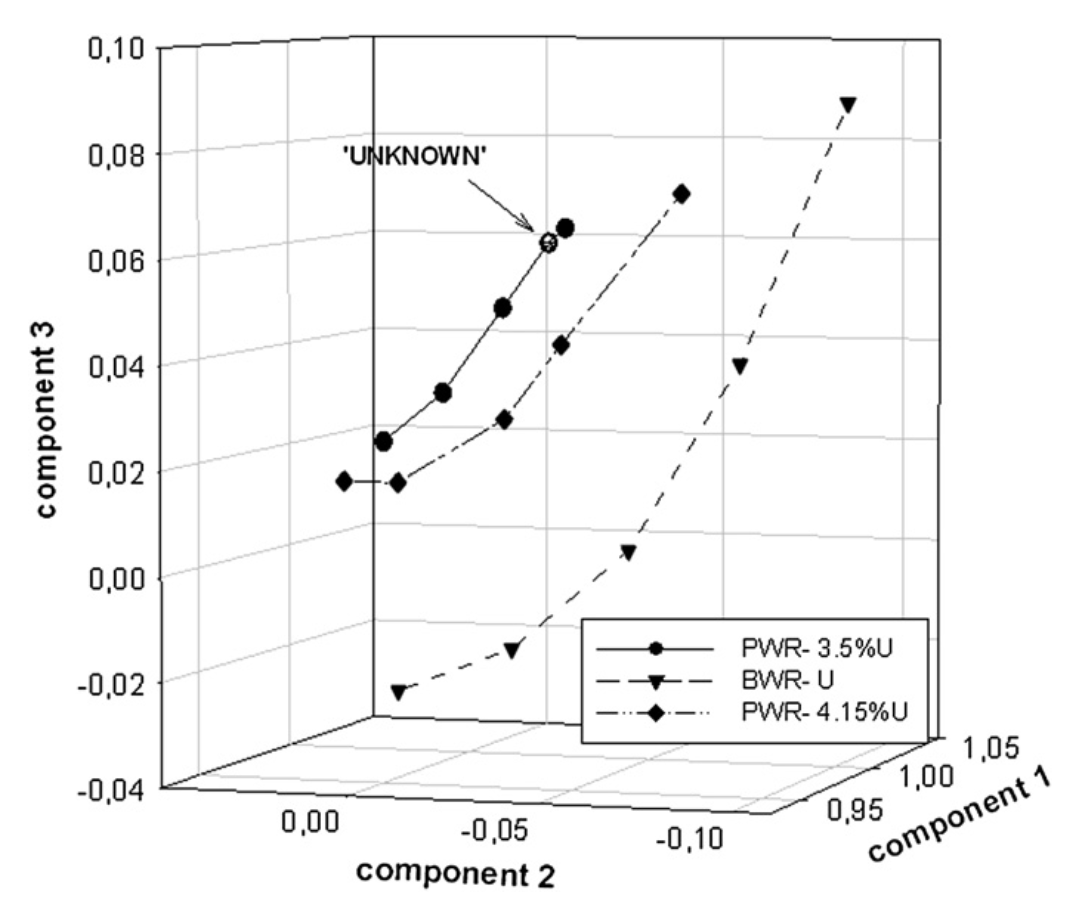
\includegraphics[width=0.5\linewidth]{./chapters/litrev/nicolaou.png}
  \caption[Example of factor analysis for \acrshort{SNF} discrimination]
          {Example from Reference \cite{nicolaou_pu} on using factor analysis
           to show similarities between classes of \acrshort{SNF} for visual 
           identification.}
  \label{fig:nico}
\end{figure}

The chronologically earliest study in this grouping of publications
\cite{nicolaou_2006} uses \gls{ORIGEN}-simulated uranium and plutonium
(${}^{234}\text{U}$, ${}^{235}\text{U}$, ${}^{236}\text{U}$,
${}^{238}\text{U}$, ${}^{238}\text{Pu}$, ${}^{239}\text{Pu}$,
${}^{240}\text{Pu}$, ${}^{241}\text{Pu}$ and ${}^{242}\text{Pu}$) of various
\gls{SNF} designations.  These simulated measurements are subject to factor
analysis and the results usually plotted.  The unknown samples in this work are
in visual alignment with the factor-analysis-determined groupings.  Reference
\cite{nicolaou_2014} extends that study (same statistical method, same list of
isotopes) to real measured samples from the \gls{SFCOMPO} database
\cite{sfcompo, valid_sfco}.  The goal here was to determine whether the factor
analysis approach could distinguish the chosen \gls{SFCOMPO} entries well, and
the results confirm the goal was achieved.  Reference \cite{nicolaou_2015} uses
three plutonium ratios (${}^{242}\text{Pu}$/${}^{240}\text{Pu}$,
${}^{238}\text{Pu}$/$\text{Pu}_{\text{Total}}$, and
${}^{239}\text{Pu}$/${}^{240}\text{Pu}$) to accomplish the same goal with
simulated \gls{SNF} without factor analysis, and the results are similar. 

This work mostly relies on actinides for identifying \gls{SNF}
\cite{nicolaou_2006, nicolaou_pu, nicolaou_2014, nicolaou_2015}, but the use of
fission products is also promising \cite{nicolaou_2009}.  This particular
publication was interesting because the author chose to use one set of fission
products to represent a typical mass spectrometry assay (${}^{133}\text{Cs}$,
${}^{140}\text{Ce}$, ${}^{150}\text{Sm}$, ${}^{152}\text{Sm}$,
${}^{144}\text{Nd}$, ${}^{145}\text{Nd}$, ${}^{146}\text{Nd}$,
${}^{148}\text{Nd}$, ${}^{150}\text{Nd}$), and another set to represent what
could be determined from a gamma detector (${}^{95}\text{Zr}$,
${}^{95}\text{Nb}$, ${}^{106}\text{Ru}$, ${}^{134}\text{Cs}$,
${}^{137}\text{Cs}$, ${}^{144}\text{Ce}$).  This approach is successful when
the simulation uncertainty is below 3\% \cite{nicolaou_2009}.

\subsection{Other Classification Work}

There are other papers on statistical methods that focus on the classification
of the reactor type for unknown samples that helped frame this work.  One study
simulated and tracked 34 nuclides of a set of typical commercial nuclear power
reactors and their operation parameters, but first used statistical
dimensionality reduction (via Laplacian eigenmaps) before subjecting the
training data to reactor type classification, comparing linear discriminant
analysis, quadratic discriminant analysis, random forests, and Parzen window
classifiers \cite{jones_snf_2014}.  Condensing the 34 features into three has
not only computational and potentially discriminatory benefits, there are
visualization benefits as shown in Figure \ref{fig:jones}.  This plot and this
work also highlights and addresses a known problem: reliable discrimination
between \gls{SNF} from \glspl{PWR} and \glspl{BWR}. 

\begin{figure}[!htb]
  \centering
  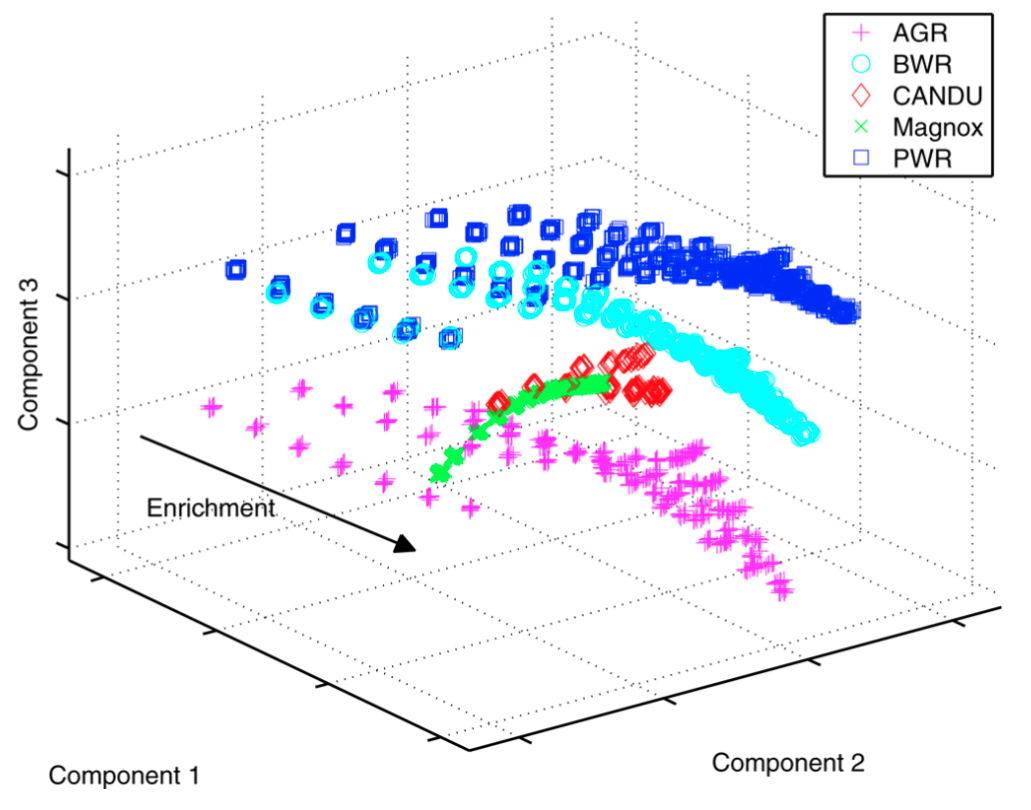
\includegraphics[width=0.7\linewidth]{./chapters/litrev/jones.png}
  \caption[Example of dimensionality reduction for visualization]
          {Results of leveraging a pre-processing step of dimensionality 
           reduction for visualization purposes, from Reference 
           \cite{jones_snf_2014}.}
  \label{fig:jones}
\end{figure}

Another paper compared principal components analysis and partial least squares
discriminant analysis to classify reactor type. As with the above, a set of
\gls{SNF} from typical commercial power reactors from around the world were
simulated and used as test samples for this attribution step, but unlike the
above they chose to focus on uranium and plutonium isotopes to address the
challenge of identifying chemically separated uranium or plutonium. This work
uses a qualitative visual distinguishability discussion to choose the better
method of partial least squares discriminant analysis.

\subsection{Regression Work}

A paper that greatly influenced the development of this study involves not only
statistical methods but an investigation of those methods when faced with
information reduction via random nuclide measurement errors in the training
data set \cite{dayman_feasibility_2013}.  Additionally, feature reduction was
investigated by using various nuclide compositions: the top 200 nuclides by
concentration in each vector, fission products only, and a principal components
analysis-derived shortened nuclide list.  

\begin{figure}[!htb]
  \centering
  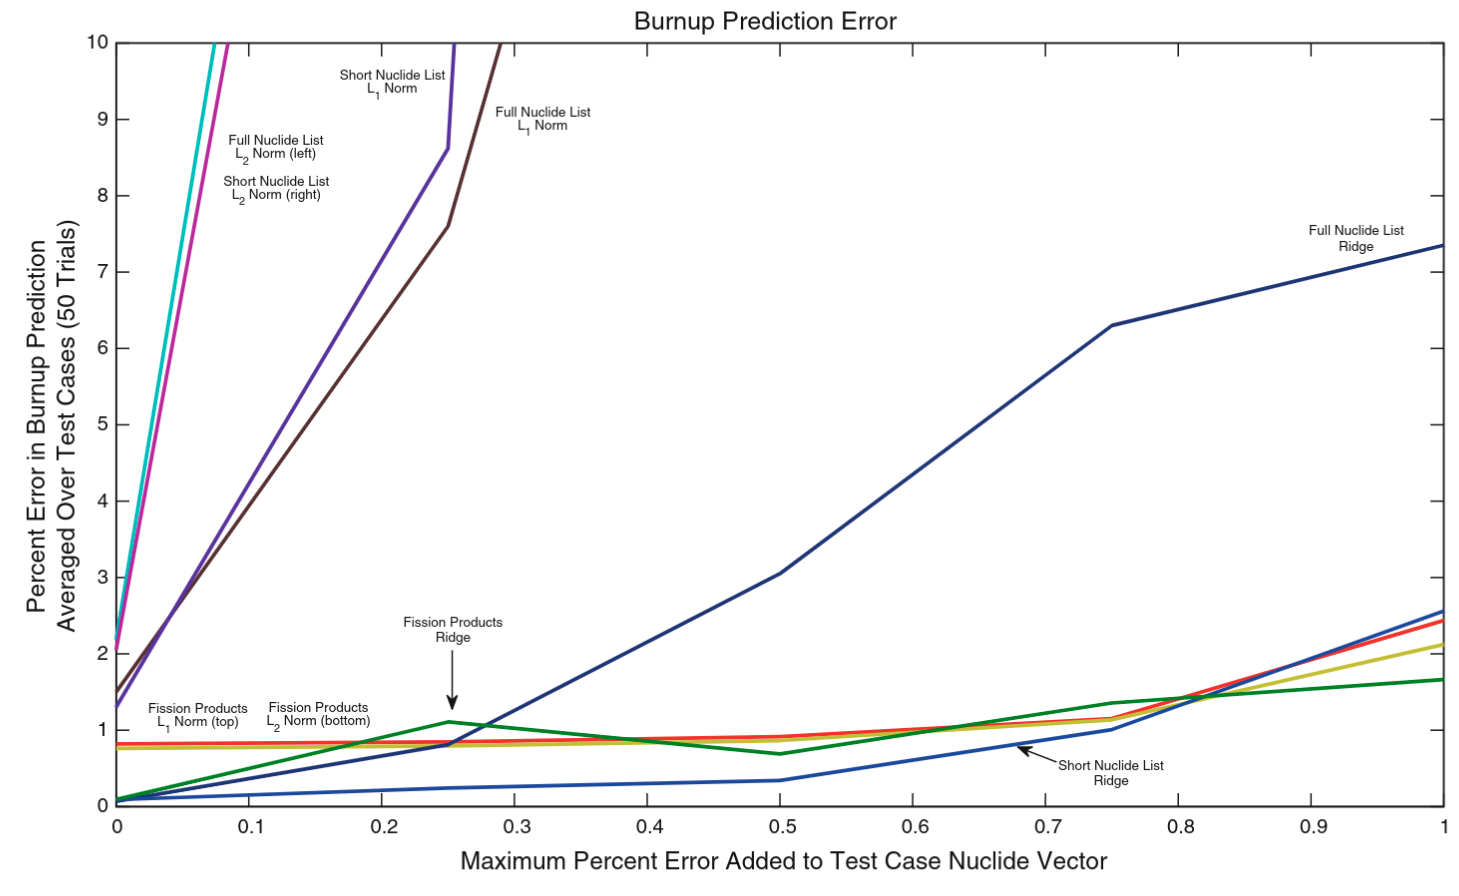
\includegraphics[width=\linewidth]{./chapters/litrev/dayman.png}
  \caption[Burnup performance with respect to training set error]
          {Plot from Reference \cite{dayman_feasibility_2013} that shows the 
           degradation of burnup prediction performance with respect to 
           increasing training set error for three algorithm implementations 
           and three feature sets.}
  \label{fig:dayman}
\end{figure}

Using these various feature sets, three methods were also compared. First and
second, the nearest neighbor algorithm with two different distance metrics was
used: Manhattan distance ($L_1$ norm, or sum of absolute differences of
Cartesian coordinates) and Euclidean distance ($L_2$ norm, or square root of
the sum of squared differences of Cartesian coordinates).  The nearest neighbor
approaches classified reactor type and predicted burnup.  Third, ridge
regression with an $L_2$ norm for regularization was only applied to burnup
prediction.  In both classification and regression cases, using the fission
products nuclide list with both nearest neighbor methods performed the best.
All other nuclide lists quickly devolved to random guesses with an increase in
nuclide error in the case of reactor prediction, and more than 100\% error in
the case of burnup prediction. Figure \ref{fig:dayman} shows the behavior of
burnup prediction at low training set error (under 1\%) for the various methods
with feature set combinations. 

\subsection{Maximum Log-Likelihood Calculations}

Another set of publications focuses on a particular methodology that was chosen
to be implemented in this work. Although many commonly used statistical methods
have been previously discussed in this section, this approach is unique: a
\gls{MLL} calculation approach for determining the similarity of a test sample
to a database of simulated samples \cite{mll_method}.  The mathematical
framework for \gls{MLL} calculations is in Section \ref{sec:algs}.  This was
developed to attribute weapons-grade plutonium, and so the training database is
only simulated with low burnup values.  Additionally, the time steps are much
smaller than what exists in the training set in this work, and these
publications focus on a set of 10 isotope ratios as the feature set.  Despite
these differences, this approach is still applicable to this work, which
focuses on \gls{SNF}. 

\begin{figure}[!htb]
  \centering
  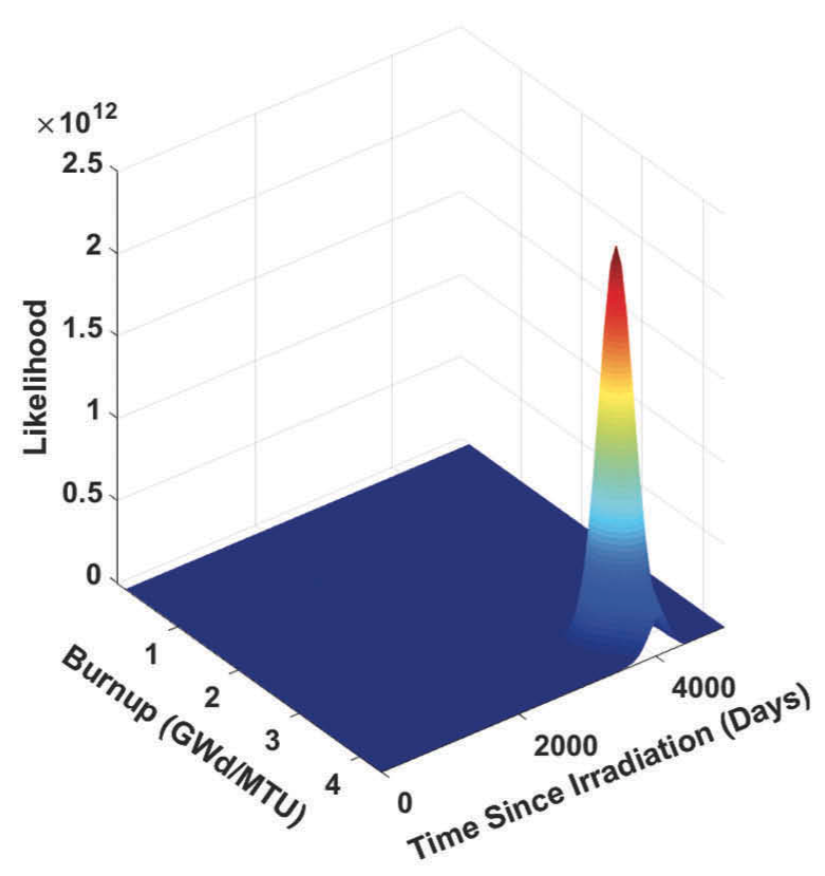
\includegraphics[width=0.6\linewidth]{./chapters/litrev/tamu.png}
  \caption[Example of likelihood maximum predicting burnup and time since 
           irradiation]
          {Plot from Reference \cite{mll_method} that shows a sample being 
           assigned burnup and time since irradiation values based on a 
           likelihood maximum.}
  \label{fig:tamu}
\end{figure}

Figure \ref{fig:tamu} shows one of the results, where a simulated sample of
$4.39\:GWd/MTU$ burnup and $3652\:days$ time since irradiation is tested
against the training database via likelihood calculations of the feature set of
10 isotope ratios; the maximum is visibly close to the ground truths.  This
method was later validated with experimental samples, in Reference
\cite{mll_validate}. 

\begin{figure}[!htb]
  \centering
  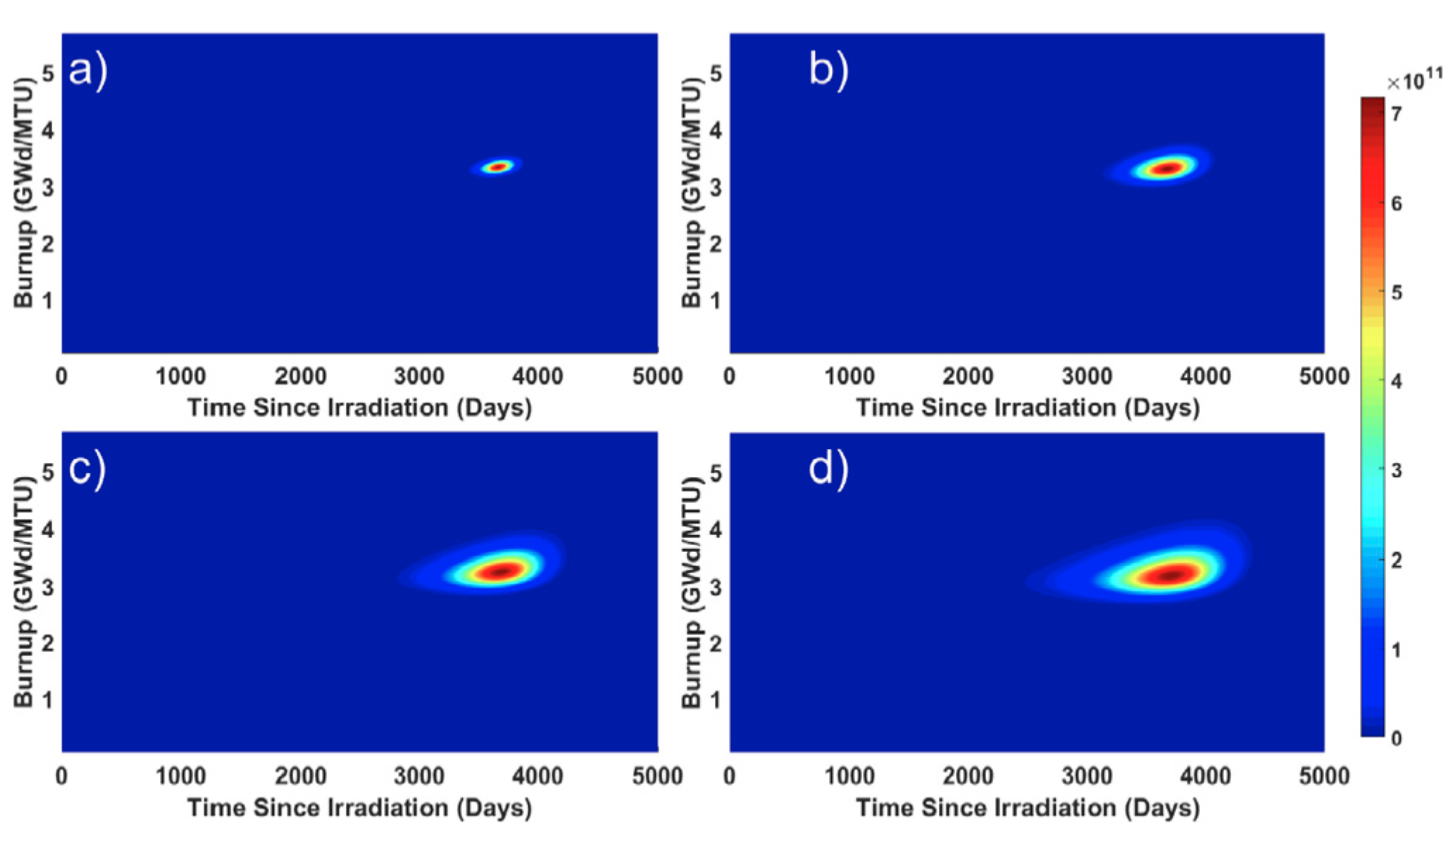
\includegraphics[width=\linewidth]{./chapters/litrev/tamu2.png}
  \caption[Sensitivity of likelihood to training set uncertainty]
          {Results from a sensitivity study on the \gls{MLL} method where 
           uncertainty of the training set was increased. The levels shown 
           here are (a) 7\%, (b) 14\%, (c) 21\%, and (d) 28\% 
           \cite{mll_sensitivity}.}
  \label{fig:tamu2}
\end{figure}

After experimental validation, sensitivity studies were conducted in Reference
\cite{mll_sensitivity}.  Figure \ref{fig:tamu2} shows a set of results from the
increasing of uncertainty. It is interesting that the likelihood decrease
happens faster on the time since irradiation axis than on the burnup axis,
since this work has also determined burnup to be easier to predict with
accuracy than time since irradiation (even with a different feature set).

\subsection{Summary}

Write me
